% !TEX TS-program = xelatex
% !TEX encoding = UTF-8 Unicode
% !Mode:: "TeX:UTF-8"

\documentclass{resume}
\usepackage{zh_CN-Adobefonts_external} % Simplified Chinese Support using external fonts (./fonts/zh_CN-Adobe/)
% \usepackage{NotoSansSC_external}
% \usepackage{NotoSerifCJKsc_external}
% \usepackage{zh_CN-Adobefonts_internal} % Simplified Chinese Support using system fonts
\usepackage{linespacing_fix} % disable extra space before next section
\usepackage{cite}
\usepackage{graphicx}
\usepackage{tabu}
\usepackage{multirow}
\usepackage{progressbar}

\begin{document}
\pagenumbering{gobble} % suppress displaying page number

\Large{
  \begin{tabu}{c  l  l}
   \multirow{4}{1in}{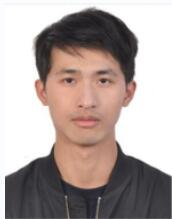
\includegraphics[width=1in]{avatar}} & \scshape{姓名:熊伟康} \\
    & \email{D1761322862wk@163.com}&年龄:21岁\\
    & \phone{(+86) 138-0353-7357}&籍贯:江西南昌\\
    & \github[github.com/xiongweikang12]{}& 意向职位:供应链专员\\
  \end{tabu}
}


\section{\faGraduationCap\  教育背景}
\datedsubsection{\textbf{东南大学成贤学院}, 南京}{2020 -- 至今}
\textit{在读本科生}\ 交通运输专业, 预计 2024 年 6 月毕业

\section{\faUsers\ 实习兼职/项目经历}

\datedsubsection{\textbf{交通预测模型和流量分配模型的封装}}{2022年10月 -- 2022年11月}
\role{python,numpy,matplotlib,scikit-learn,Networkx}{个人项目}
\begin{itemize}
  \item 使用面向对象多态思想
  \item 实现交通预测,交通分类等模块
  \item 对交通数据进行分析并且实现可视化
\end{itemize}

\datedsubsection{\textbf{肉类供应商实习}}{2022年12月 -- 2023年2月}
\role{}{实习}
\begin{itemize}
  \item 对订单进行核实,与保证配送时效
  \item 在月底跟配送方对账,核对货款
  \item 对货款数据进行分析,并且实现可视化呈现
  \item 处理沟通解决来自客户订单上的问题
\end{itemize}





% Reference Test
%\datedsubsection{\textbf{Paper Title\cite{zaharia2012resilient}}}{May. 2015}
%An xxx optimized for xxx\cite{verma2015large}
%\begin{itemize}
%  \item main contribution
%\end{itemize}

\section{\faCogs\ 技能}
% increase linespacing [parsep=0.5ex]
\begin{itemize}[parsep=0.5ex]
  \item 办公软件:word,excel,ppt
  \item 编程语言:C/C++,python,SQL
  \item 文本工具及版本控制工具:LaTeX,git
  \item 交通物流管理类课程:运筹学,交通数据分析,交通规划,
  \item 计算机课程:数据结构和算法,计算机组成原理,计算机网络,操作系统,程序设计,数据库系统概论。
\end{itemize}

\section{\faHeartO\ 获奖证书}
\datedline{CTE-4}{}
\datedline{机动车驾驶证}{}
\datedline{东南大学成贤学院2022蓝桥杯(软件类)热身赛}{}
\datedline{考研数学:122/150}{}

\section{\faInfo\ 其他}
% increase linespacing [parsep=0.5ex]
\begin{itemize}[parsep=0.5ex]
  \item 自我评价: 容易接受新事物,能自主的积极处理问题,学习快,对擅长数据分析,做事细心,肯吃苦,乐于与人沟通。
\end{itemize}

%% Reference
%\newpage
%\bibliographystyle{IEEETran}
%\bibliography{mycite}
\end{document}
